\subsection{Interpolation Methods}
There are several, distinct differences between the various interpolation methods implemented in our project.

The most basic interpolation method is \textit{Nearest Neighbor} which was discussed in detail in \autoref{subsec:nearest-neighbor}.
While it has very good performance, it tends to result in a loss of detail. It is able to result in sharper images however, as it does not calculate missing values, and uses the values from the original image, so this sharpness becomes a trade-off for blocky artifcating.

To contrast this, we have \textit{Bilinear} (\autoref{subsec:bilinear}) which attempts to ``fill in the gaps'' of missing data. As such, it is more computationally expensive as it involves a calculation on three points for each pixel. This results in finer detail, but can also result in blurrier images. It also tends to leave cross artifacts as opposed to the blocky artifacts from \textit{Nearest Neighbor}, though these are much less noticeable.

\textit{Bicubic} interpolation (\autoref{subsec:bicubic}) requires significant computational processing, so it is not always feasible to use for very large images. However, the quality of the images that result is noticeable, especially at high zooms. It does not have the same artifcating issue that \textit{Bilinear} has, and while still a bit blurry, is much smoother overall.

The various artifacting elements mentioned here are most noticeable along edges.  Flat/smooth surfaces, solid colors or repeating textures, like a wall, the sky, or a persons cheek won't have as noticeable of an artifacting effect because the ``guess'' that the interpolation makes is relatively close to what would actually be there if we had zoomed in.  The blue color of the sky won't change as often or as drastically as the edge of a person's smile, so we won't notice any missing values as easily.

\begin{figure}[H]
    \centering
    \subfloat[Nearest Neighbor]{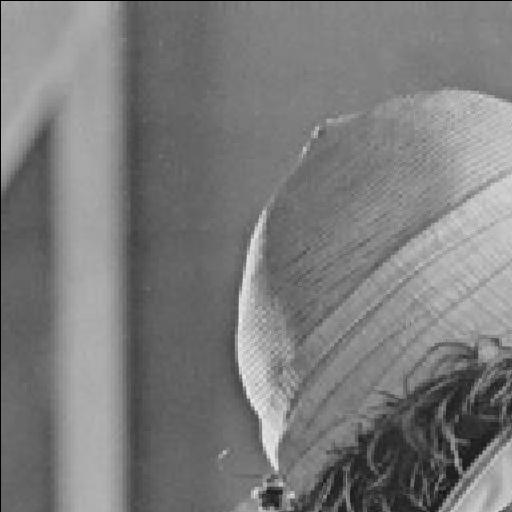
\includegraphics[width=0.4\textwidth]{images/lenna-nearest-neighbor-zoom.jpg}}
    \qquad
    \subfloat[Bilinear]{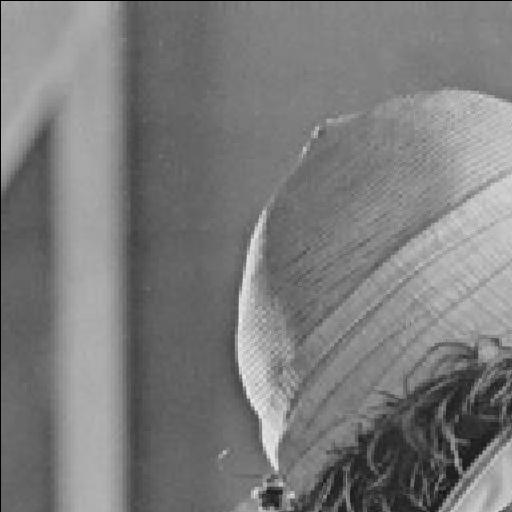
\includegraphics[width=0.4\textwidth]{images/lenna-bilinear-zoom.jpg}}
    \qquad\\
    \subfloat[Bicubic]{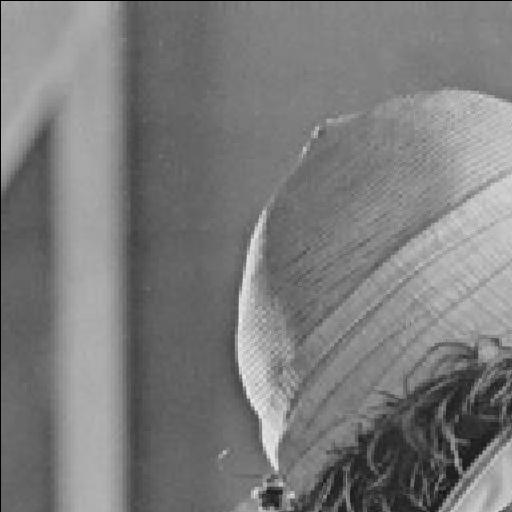
\includegraphics[width=0.4\textwidth]{images/lenna-bicubic-zoom.jpg}}
    \qquad
    \subfloat[Lanczos]{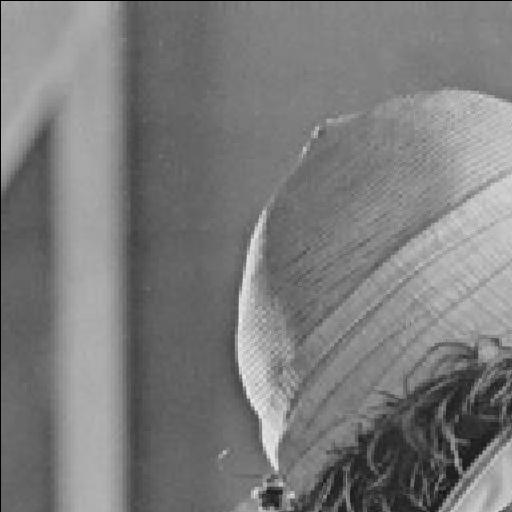
\includegraphics[width=0.4\textwidth]{images/lenna-lanczos4-zoom.jpg}}
    \caption{Side-by-Side comparison of zoomed-in interpolated images with scale $(2, 2)$}
    \label{fig:comparison}
\end{figure}